\subsection{Descri\c c\~ao do problema} \label{subsec:descricao}

A descrição do problema é fundamental para obter uma compreensão mais precisa do que está sendo abordado neste trabalho. É por meio dessa descrição que as variáveis-chave são expostas e o objetivo da previsão é estabelecido de forma clara. Sem um plano estruturado para determinar o que deve ser previsto, torna-se difícil justificar o uso de modelos de previsão de dados. Portanto, é essencial estabelecer um propósito claro e definir as metas da previsão antes de aplicar os modelos adequados.

\begin{itemize}
	\item Bombas de sucção (B1, B2 e B3) – valor máximo da frequência 60 Hz
	
	\item[] Variáveis importantes: Fluxo, pressão e nível
	
	\item Nível do Reservatório (Câmara 1) LT01 $ (m^3) $ - \textbf{PREVER}
	
	\item Vazão de entrada (FT01) $ (m^3/h) $
	
	\item Vazão de gravidade (FT02) $ (m^3/h) $
	
	\item Vazão de recalque (FT03) $ (m^3/h) $
	
	\item Pressão de Sucção (PT01SU) (mca)
	
	\item Pressão de Recalque (PT02RBAL) (mca)
\end{itemize}

A pesquisa fará uso da variável LT01, que representa o nível do reservatório e desempenha um papel de extrema importância, como evidenciado pelas Figuras \ref{fig:dados-todos} e \ref{fig:2020-a-frente}. Essas figuras retratam as anomalias ocorridas durante o período em que a capital paranaense foi afetada pela escassez de chuvas, resultando na redução do nível dos reservatórios e na implementação de rodízios periódicos, conforme discutido na subseção \ref{subsubsec:motivacao}. Assim, tais observações permitem uma compreensão mais aprofundada das perspectivas futuras.

\subsection{Procedimentos metodol{\'o}gicos} \label{subsec:metod}

Com o intuito de realizar previsões e fazer comparações entre os modelos obtidos na revisão sistemática, será adotado um processo metodológico bem definido. Tal processo está detalhado na subseção \ref{subsubsec:etp} desta seção, onde foram estabelecidas as etapas a serem seguidas desde o início. Isso inclui a definição do que será previsto, bem como a seleção dos métodos a serem utilizados na Análise Exploratória de Dados (EDA), seguindo uma sequência lógica e coerente.
   
    \subsubsection{Etapas da pesquisa}\label{subsubsec:etp}

    
    A pesquisa seguiu as seguintes etapas:
    \begin{figure}[H]
    	\centering
    	\caption{Mapa das Etapas}
    	\label{fig:etapas}
    	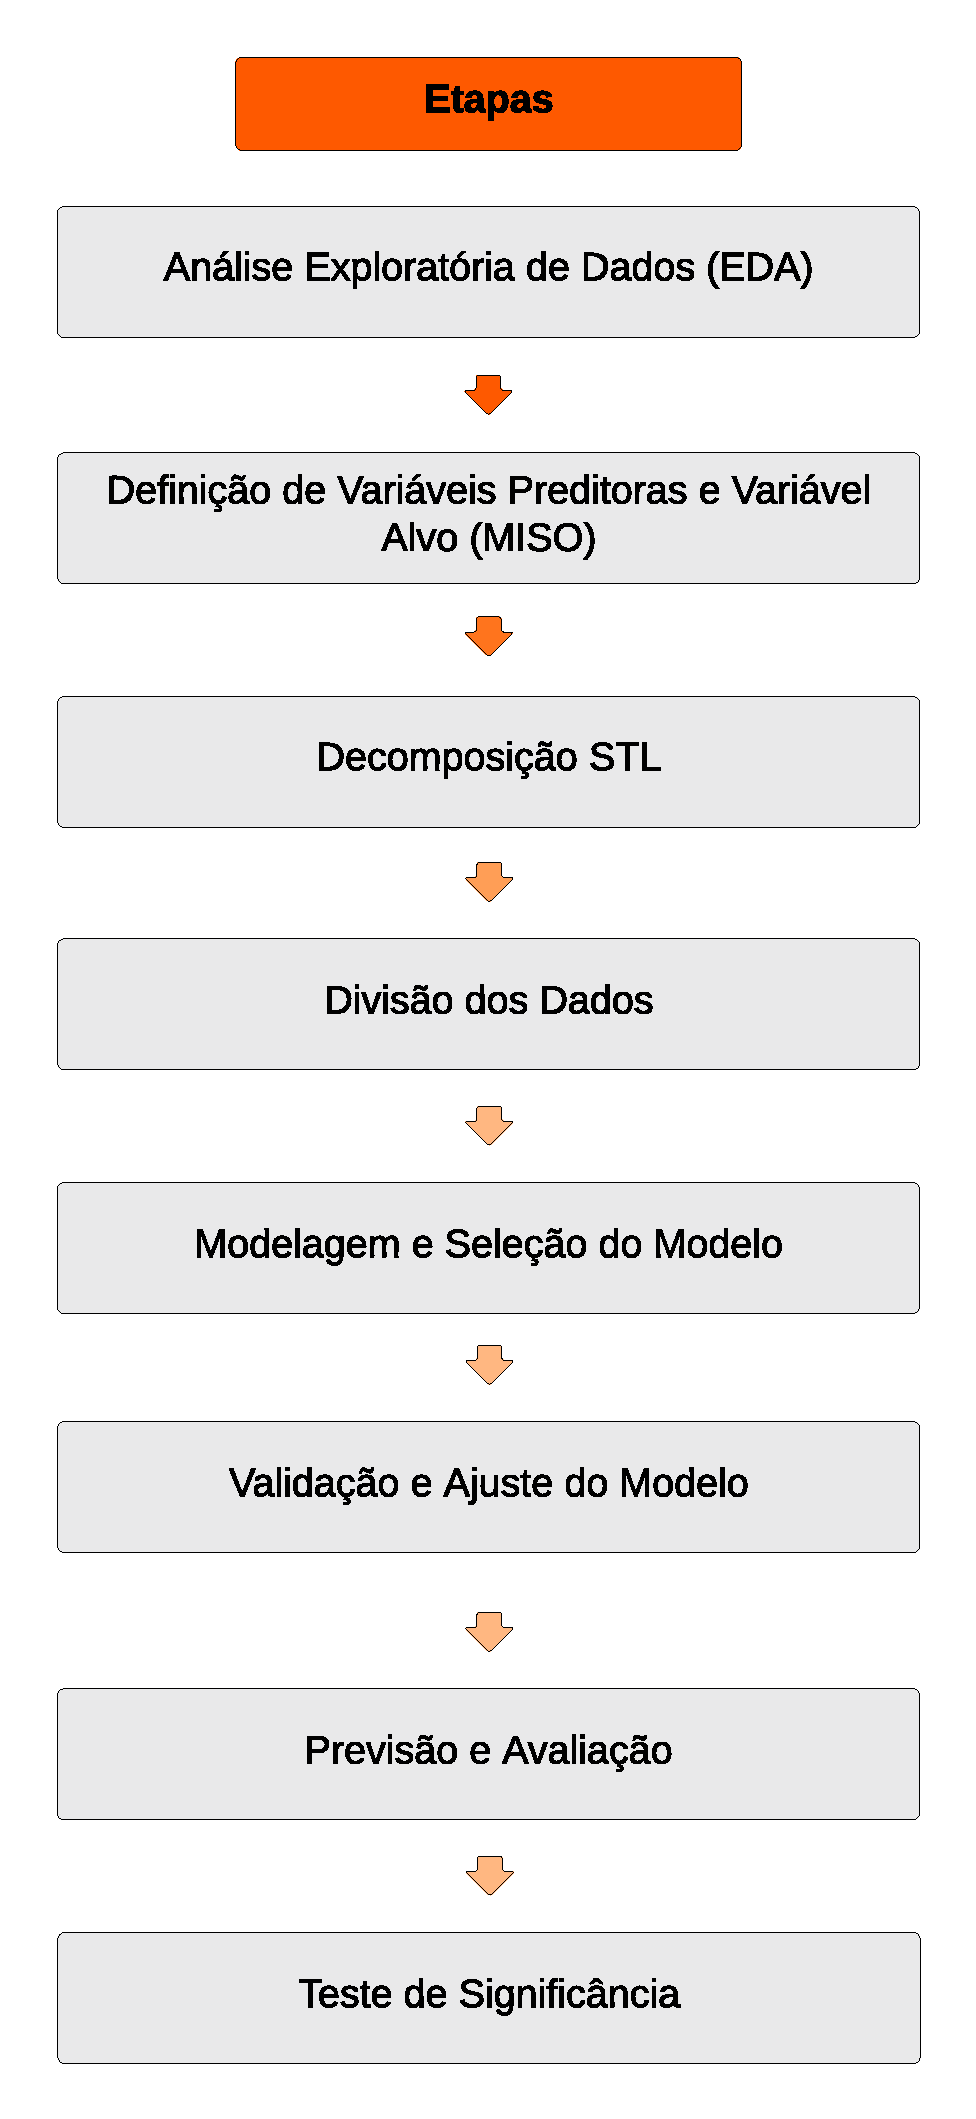
\includegraphics[width=0.9\linewidth]{Introducao/Figuras/Etapas}
    	
    	\fonte{Elaboração própria}
    \end{figure}
    \begin{enumerate}[start=1, label = {\textbf{Etapa} \arabic*} ]
    	\item Análise exploratória dos dados – EDA ( do inglês \textit{Exploratory Data Analysis}). \label{etp:1}
    	
    	A exploração de dados na EDA é fundamental para entender melhor os dados que estão sendo trabalhados, como, por exemplo, excluir valores ausentes, saber como os dados estão separados em horas ou dias e, assim, tomar a melhor decisão a ser trabalhada com os dados, usar gráficos de linha na análise para observar a convergência dos dados e as anomalias que podem ocorrer.
    	
        	
    	\item O que vai ser usado como variáveis previsoras e qual será a variável a ser predita (MISO). \label{etp:2}
    	
    	Nessa etapa, tem o papel de relacionar as variáveis ao que será previsto, como os modelos de variáveis exógenas que são usados aqui nos modelos SARIMAX, ARX e ARIMAX do tipo ARIMA. Cada modelo tem a interação de mais variáveis do que o modelo ARIMA básico ou seus derivados AR, MA e SARIMA. O conhecimento de quais variáveis estão incluídas na modelagem do problema torna a modelagem mais abrangente quando o horizonte de previsão é estendido além dos dados.
    	
       	
    	\item Fazer a decomposição STL (do inglês \textit{Seasonal-Trend Decomposition}) Sazonalidade, Tendência e Resíduo. \label{etp:3}
    	
    	\citeonline{en15165875} destacam que ``o uso do método de decomposição STL em conjunto com um modelo híbrido se mostrou eficaz na previsão de carga de curto prazo'' (p. 6).
    	
    	Segundo \citeonline{inproceedings}, ``a aplicação da decomposição STL e do modelo LSTM baseado em atenção foi capaz de prever com precisão a velocidade do tráfego de curto prazo'' (p. 6).
    	
    	\citeonline{su13041694} afirmam que ``a combinação da decomposição STL e modelos de aprendizado profundo mostrou-se promissora na previsão de carga de eletricidade'' (p. 18).
    	
        O algoritmo STL executa suavização na série de tempo usando LOESS em dois loops; o loop interno itera entre a suavização sazonal e de tendência e o loop externo minimiza o efeito de valores atípicos. Durante o loop interno, o componente sazonal é calculado primeiro e removido para calcular o componente de tendência. O restante é calculado subtraindo os componentes sazonais e de tendência da série de tempo.
        
        Os três componentes da análise STL se relacionam com a série de tempo bruta da seguinte forma:
        
        \begin{align}
        	y_i &= s_i + t_i + r_i\label{eq:stl1}
        \end{align}
    	
    	Da equação \eqref{eq:stl1}:
    	
    	\begin{itemize}
    		\item $y_i = O$ valor da série de tempo no ponto $i$.
    		\item $s_i = O$ valor do componente sazonal no ponto $i$.
    		\item $t_i = O$ valor do componente de tendência no ponto $i$.
    		\item $ri = O$ valor do componente restante no ponto $i$.
    	\end{itemize}
    	\item \label{etp:4} Separação dos dados.
    	
  
    De acordo com a literatura acadêmica, é comum dividir o conjunto de dados em treinamento, validação e teste para avaliar a performance dos modelos. Essa abordagem permite uma análise mais completa do desempenho do modelo, garantindo uma avaliação objetiva de sua capacidade de generalização e evitando problemas de overfitting ou subajuste \cite{cruz-ramirez2020enhancing,mokhtari2020deep,khan2021hybrid,sharma2021deep}.
    
    A fim de obter uma divisão mais adequada dos dados, é realizado um estudo das medidas de tendência central e dispersão de cada conjunto. O conjunto de dados é então dividido em três partes distintas: treinamento, validação e teste. Nessa divisão, inicialmente, 70\% dos dados são utilizados para o treinamento e validação, enquanto os 30\% restantes são reservados para o conjunto de teste. Em seguida, a porção destinada ao treinamento e validação é subdividida em uma proporção de 80\% para treinamento e 20\% para validação.
    	
    	
    	\item Estratégia de previsão (recursiva e iterada-método direto). \label{etp:5}
    	
    	A estratégia recursiva é mencionada por \citeonline{PETROPOULOS2022705} como uma abordagem eficaz na previsão de séries temporais de múltiplos passos. De acordo com o autor, essa estratégia envolve o uso de previsões anteriores como entradas para prever os próximos passos da série temporal. A abordagem recursiva tem demonstrado potencial para melhorar a acurácia das previsões de séries temporais de longo prazo.
    	
    	A estratégia recursiva consiste em utilizar um modelo de previsão de um passo de tempo várias vezes, onde a previsão obtida no passo anterior é utilizada como entrada para realizar a previsão do próximo passo de tempo.
    	
    	No contexto da previsão da demanda de água para os próximos dias, seria desenvolvido um modelo de previsão de um único passo. Esse modelo seria aplicado para prever a demanda no primeiro dia e, em seguida, essa previsão seria utilizada como dado de entrada para prever a demanda do segundo dia. Esse processo se repetiria para os demais dias, permitindo a previsão da demanda ao longo do tempo.
    	    		 
    	Por Exemplo:
    	
    	\begin{eqnarray}
    	preditivo(t+1) &=& model_1(obs(t-1), obs(t-2), \ldots, obs(t-n))\\
    	preditivo(t+2) &=& model_2(obs(t-2), obs(t-3), \ldots, obs(t-n))   	
    	\end{eqnarray}
    	
    	\citeonline{machinemaster} como as previsões são usadas no lugar das observações, a estratégia recursiva permite que os erros de previsão se acumulem de tal forma que o desempenho possa se degradar rapidamente à medida que o horizonte de tempo de previsão aumenta.
    	
    	
    	\item Horizonte de previsão (1 passo ou n passos à frente). \label{etp:6}
    	
    	Para abordar a diversidade de horizontes de previsão, optou-se por considerar diferentes intervalos de tempo. Isso permitirá a realização de previsões para um passo à frente, uma semana, duas semanas e um mês, de forma a abranger distintas perspectivas de curto e médio prazo. Essa abordagem proporciona uma análise abrangente da capacidade dos modelos em lidar com horizontes de previsão variados, contribuindo para uma avaliação mais completa e precisa do desempenho dos mesmos.
    	
    	
    	\item Modelos de previsão e métricas de desempenho. \label{etp:7}
    	
    	Os modelos abordados nesta pesquisa são tanto os modelos clássicos de previsão quanto os modelos de regressão por gradiente. Entre os modelos clássicos, incluem-se o AR, ARX, ARMA, ARIMA, SARIMA, SARIMAX e ARIMAX, enquanto os modelos de regressão por gradiente englobam o LR, XGBRegressor, RFR e LGBMRegressor. A seleção desses modelos foi baseada em uma revisão sistemática realizada durante a dissertação, buscando identificar os modelos mais eficazes e amplamente utilizados na literatura.
    	
    	Ao longo da pesquisa, foram adotadas três métricas principais para avaliar o desempenho dos modelos: RRMSE, MAE  e sMAPE. Essas métricas foram escolhidas com base na revisão sistemática e são amplamente reconhecidas como medidas de qualidade de previsão. Cada métrica tem sua própria interpretação e importância, sendo detalhada na subseção \ref{subsec:metrica} para um melhor entendimento de como são aplicadas e interpretadas na pesquisa.
    	
    	
    	
    	%\item Ajustar os hiperparâmetros dos modelos de previsão Hiperparâmetro ajusta a priori (ex: número de neurônios da rede neural), e parâmetro (pesos da rede neural) ajusta durante o processo. \label{etp:8}
    	
    	
    	\item Aplicar os modelos de previsão e fazer comparativo baseado em testes de significância estatística (\textit{Friedman e Nemenyi}). \label{etp:9}
    	
    	
    	O teste de Friedman é o teste não paramétrico usado para comparar dados de amostras vinculadas, ou seja, quando o mesmo indivíduo é avaliado mais de uma vez. 
    	ou seja, quando o mesmo indivíduo é avaliado mais de uma vez. 
    	O teste de Friedman não usa os dados numéricos diretamente, mas sim as classificações ocupadas pelos dados após a classificação de cada grupo separadamente. 
    	separadamente. Após a classificação, a hipótese de igualdade da soma das classificações de cada grupo é testada. 

		O teste consiste em fazer comparações em pares com o intuito de verificar qual dos fatores que diferem entre si. No entanto, o teste de Nemenyi é muito conservador e pode não encontrar diferença significativa entre os pares testados.
    	
    \end{enumerate}






    